\subsection{Fundamental Particles and Interactions}
\label{sec:Intro_FundParticles}

\begin{figure}[htb]
  \begin{center}
    {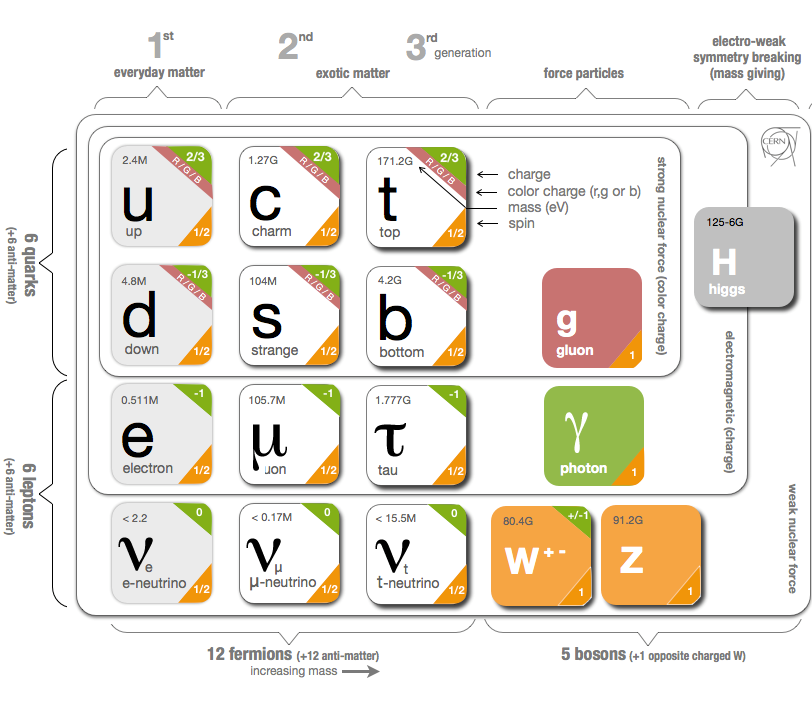
\includegraphics[width=0.90\textwidth]{../figs/Intro/StandardModel.png}}
    \caption{Standard Model Particles and Interations}
    \label{fig:SMtable}
  \end{center}
\end{figure}

The SM particles and summarized in Fig. \ref{fig:SMtable}. 

The fermions are arranged into three generations, each generation consists of a quark with charge Q=+2/3(up, charm and top quarks), a quark with Q=-1/3 (down, strange and bottom quarks), a lepton with Q=-1 (electron, muon, tau-lepton) and a neutrino which is electrically neutral. (The unit of the electric charge used is an absolute value of an electron charge). Higher generation particles have larger masses compared to the corresponding low generation particles. 

In addition to fermions, the SM include four bosons which are mediators for the SM interactions. Gluons are mediators of the strong interactions. Only quarks, antiquarks and gluons can participate in the strong interactions. These particles possess a special quantum number - the color charge. Quarks can be red, green or blue (although these are just names of the properties, not actual colors). Antiquarks can be antired, antigreen or antiblue. 

Photon is a mediator for the electromagnetic interactions. All electrically charged particles participate in electromagnetic interactions. W$^{\pm}$ and Z$^0$ bosons are mediators of the weak interactions. All particles participate in weak interactions. W$^{\pm}$ and Z$^0$ bosons are massive while photon and gluon are massless particles. 

The Higgs boson is the boson which is responsible for W and Z bosons to get masses.

All the particles are listed in Fig. \ref{fig:SMtable}. These and only these fundamental particles have been discovered by now (and their antiparticles). However, there are many composite particles which are called hadrons. Hadrons can consist of three quarks (baryons), quark and antiquark (meson), or three antiquarks (antibaryons). Hadrons always possess an integer charge and are colorless.

Protons and neutrons are baryons.

Most of the particles are short-lived and decay into lighter particles within microseconds. The only stable particles (in terms that they do not decay) are protons and antiprotons, electrons and positrons, neutrinos and antineutrinos, photons and gluons. However, if a particle can not decay, it does not mean that  it would live forever. Antiprotons and positrons would immediately annihilate in the presence of a substance, and color-charged free gluons can not exist.

In addition to the three fundamental forces mentioned above, there is also the fourth one: the gravity. It is not included into the SM but its effect on particles is negligible compared to the other forces which makes it possible to develop theory and conduct experiments of particles physics even without having the gravity included into the model.

%%The electromagnetic and weak interactions are discussed in more details in Sec. \ref{sec:Intro_Electroweak} with the Higgs mechanism explained in \ref{sec:Intro_Higgs} and the strong interactions are discussed in more details in Sec. \ref{sec:Intro_QCD}. In addition to these three interaction, there is the fourth fundamental interaction known: the gravity. The gravity is not included into the SM.


